% SIAM Article Template
\documentclass[review,hidelinks,onefignum,onetabnum]{siamart220329}

% Information that is shared between the article and the supplement
% (title and author information, macros, packages, etc.) goes into
% ex_shared.tex. If there is no supplement, this file can be included
% directly.

% SIAM Shared Information Template
% This is information that is shared between the main document and any
% supplement. If no supplement is required, then this information can
% be included directly in the main document.


% Packages and macros go here
\usepackage{lipsum}
\usepackage{amsfonts}
\usepackage{graphicx}
\usepackage{epstopdf}
\usepackage{algorithmic}
\ifpdf
  \DeclareGraphicsExtensions{.eps,.pdf,.png,.jpg}
\else
  \DeclareGraphicsExtensions{.eps}
\fi

% Add a serial/Oxford comma by default.
\newcommand{\creflastconjunction}{, and~}

% Used for creating new theorem and remark environments
\newsiamremark{remark}{Remark}
\newsiamremark{hypothesis}{Hypothesis}
\crefname{hypothesis}{Hypothesis}{Hypotheses}
\newsiamthm{claim}{Claim}

% Sets running headers as well as PDF title and authors
\headers{An Example Article}{D. Doe, P. T. Frank, and J. E. Smith}

% Title. If the supplement option is on, then "Supplementary Material"
% is automatically inserted before the title.
\title{Fast Matrix composition of Pauli polynomial
\thanks{Submitted to the editors DATE.
\funding{This work was funded by the Fog Research Institute under contract no.~FRI-454.}}}

% Authors: full names plus addresses.
\author{Dianne Doe\thanks{Imagination Corp., Chicago, IL 
  (\email{ddoe@imag.com}, \url{http://www.imag.com/\string~ddoe/}).}
\and Paul T. Frank\thanks{Department of Applied Mathematics, Fictional University, Boise, ID 
  (\email{ptfrank@fictional.edu}, \email{jesmith@fictional.edu}).}
\and Jane E. Smith\footnotemark[3]}

\usepackage{amsopn}
\DeclareMathOperator{\diag}{diag}


%%% Local Variables: 
%%% mode:latex
%%% TeX-master: "ex_article"
%%% End: 


% Optional PDF information
\ifpdf
\hypersetup{
  pdftitle={An Example Article},
  pdfauthor={D. Doe, P. T. Frank, and J. E. Smith}
}
\fi

% The next statement enables references to information in the
% supplement. See the xr-hyperref package for details.

\externaldocument[][nocite]{ex_supplement}

% FundRef data to be entered by SIAM
%<funding-group specific-use="FundRef">
%<award-group>
%<funding-source>
%<named-content content-type="funder-name"> 
%</named-content> 
%<named-content content-type="funder-identifier"> 
%</named-content>
%</funding-source>
%<award-id> </award-id>
%</award-group>
%</funding-group>

\begin{document}

\maketitle

% REQUIRED
\begin{abstract}
This is an example SIAM \LaTeX\ article. This can be used as a
template for new articles.  Abstracts must be able to stand alone
and so cannot contain citations to the paper's references,
equations, etc.  An abstract must consist of a single paragraph and
be concise. Because of online formatting, abstracts must appear as
plain as possible. Any equations should be inline.
\end{abstract}

% REQUIRED
\begin{keywords}
example, \LaTeX
\end{keywords}

% REQUIRED
\begin{MSCcodes}
68Q25, 68R10, 68U05
\end{MSCcodes}

\section{Introduction}
The introduction introduces the context and summarizes the
manuscript. It is importantly to clearly state the contributions of
this piece of work. The next two paragraphs are text filler,
generated by the \texttt{lipsum} package.

\lipsum[2-3]

% The outline is not required, but we show an example here.
The paper is organized as follows. Our main results are in
\cref{sec:main}, our new algorithm is in \cref{sec:alg}, experimental
results are in \cref{sec:experiments}, and the conclusions follow in
\cref{sec:conclusions}.

\section{Main results}
\label{sec:main}

We interleave text filler with some example theorems and theorem-like
items.

\lipsum[4]

Here we state our main result as \cref{thm:bigthm}; the proof is
deferred to \cref{sec:proof}.

\begin{theorem}[$LDL^T$ Factorization \cite{GoVa13}]\label{thm:bigthm}
  If $A \in \mathbb{R}^{n \times n}$ is symmetric and the principal
  submatrix $A(1:k,1:k)$ is nonsingular for $k=1:n-1$, then there
  exists a unit lower triangular matrix $L$ and a diagonal matrix
  \begin{displaymath}
    D = \diag(d_1,\dots,d_n)
  \end{displaymath}
  such that $A=LDL^T$. The factorization is unique.
\end{theorem}

\lipsum[6]

\begin{theorem}[Mean Value Theorem]\label{thm:mvt}
  Suppose $f$ is a function that is continuous on the closed interval
  $[a,b]$.  and differentiable on the open interval $(a,b)$.
  Then there exists a number $c$ such that $a < c < b$ and
  \begin{displaymath}
    f'(c) = \frac{f(b)-f(a)}{b-a}.
  \end{displaymath}
  In other words,
  \begin{displaymath}
    f(b)-f(a) = f'(c)(b-a).
  \end{displaymath}
\end{theorem}

Observe that \cref{thm:bigthm,thm:mvt,cor:a} correctly mix references
to multiple labels.

\begin{corollary}\label{cor:a}
  Let $f(x)$ be continuous and differentiable everywhere. If $f(x)$
  has at least two roots, then $f'(x)$ must have at least one root.
\end{corollary}
\begin{proof}
  Let $a$ and $b$ be two distinct roots of $f$.
  By \cref{thm:mvt}, there exists a number $c$ such that
  \begin{displaymath}
    f'(c) = \frac{f(b)-f(a)}{b-a} = \frac{0-0}{b-a} = 0.
  \end{displaymath}
\end{proof}

Note that it may require two \LaTeX\ compilations for the proof marks
to show.

Display matrices can be rendered using environments from \texttt{amsmath}:
\begin{equation}\label{eq:matrices}
S=\begin{bmatrix}1&0\\0&0\end{bmatrix}
\quad\text{and}\quad
C=\begin{pmatrix}1&1&0\\1&1&0\\0&0&0\end{pmatrix}.
\end{equation}
Equation \cref{eq:matrices} shows some example matrices.

We calculate the Fr\'{e}chet derivative of $F$ as follows:
\begin{subequations}
\begin{align}
  F'(U,V)(H,K) 
  &= \langle R(U,V),H\Sigma V^{T} + U\Sigma K^{T} -
  P(H\Sigma V^{T} + U\Sigma K^{T})\rangle \label{eq:aa} \\
  &= \langle R(U,V),H\Sigma V^{T} + U\Sigma K^{T}\rangle 
  \nonumber \\
  &= \langle R(U,V)V\Sigma^{T},H\rangle + 
  \langle \Sigma^{T}U^{T}R(U,V),K^{T}\rangle. \label{eq:bb}
\end{align}
\end{subequations}
\Cref{eq:aa} is the first line, and \cref{eq:bb} is the last line.

\section{Algorithm}
\label{sec:alg}

\lipsum[40]

Our analysis leads to the algorithm in \cref{alg:buildtree}.

\begin{algorithm}
\caption{Build tree}
\label{alg:buildtree}
\begin{algorithmic}
\STATE{Define $P:=T:=\{ \{1\},\ldots,\{d\}$\}}
\WHILE{$\#P > 1$}
\STATE{Choose $C^\prime\in\mathcal{C}_p(P)$ with $C^\prime := \operatorname{argmin}_{C\in\mathcal{C}_p(P)} \varrho(C)$}
\STATE{Find an optimal partition tree $T_{C^\prime}$ }
\STATE{Update $P := (P{\setminus} C^\prime) \cup \{ \bigcup_{t\in C^\prime} t \}$}
\STATE{Update $T := T \cup \{ \bigcup_{t\in\tau} t : \tau\in T_{C^\prime}{\setminus} \mathcal{L}(T_{C^\prime})\}$}
\ENDWHILE
\RETURN $T$
\end{algorithmic}
\end{algorithm}

\lipsum[41]

\section{Experimental results}
\label{sec:experiments}

\lipsum[50]

\Cref{fig:testfig} shows some example results. Additional results are
available in the supplement in \cref{tab:foo}.

\begin{figure}[htbp]
  \centering
  \label{fig:a}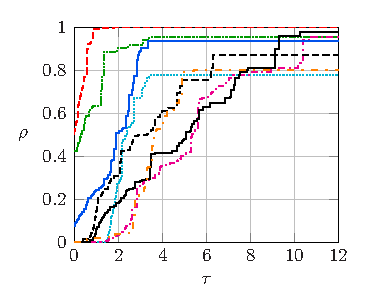
\includegraphics{lexample_fig1}
  \caption{Example figure using external image files.}
  \label{fig:testfig}
\end{figure}

\Cref{tab:foo} shows additional
supporting evidence. 

\begin{table}[htbp]
\footnotesize
\caption{Example table.}\label{tab:foo}
\begin{center}
  \begin{tabular}{|c|c|c|} \hline
   Species & \bf Mean & \bf Std.~Dev. \\ \hline
    1 & 3.4 & 1.2 \\
    2 & 5.4 & 0.6 \\ 
    3 & 7.4 & 2.4 \\ 
    4 & 9.4 & 1.8 \\ \hline
  \end{tabular}
\end{center}
\end{table}

\lipsum[51]

\section{Discussion of \texorpdfstring{{\boldmath$Z=X \cup Y$}}{Z = X union Y}}

\lipsum[76]

\section{Conclusions}
\label{sec:conclusions}

Some conclusions here.


\appendix
\section{An example appendix} 
\lipsum[71]

\begin{lemma}
Test Lemma.
\end{lemma}


\section*{Acknowledgments}
We would like to acknowledge the assistance of volunteers in putting
together this example manuscript and supplement.

\bibliographystyle{siamplain}
\bibliography{references}
\end{document}
